\setcounter{figure}{0}
\setcounter{table}{0}
\setcounter{page}{1}
\renewcommand{\thefigure}{Supp.~Fig.~\arabic{figure}}
\renewcommand{\thetable}{Supp.~Table~\arabic{table}}
\renewcommand{\thepage}{S\arabic{page}}
  
%%% TITLE %%%
\title{\Large \bf Supplementary Information: Canalization of the evolutionary trajectory of the human influenza virus}
\maketitle

\section*{Supplementary methods}

\subsection*{Parameter selection and sensitivity analysis}

Estimating what the basic reproductive number $R_0$ for seasonal influenza would be in a naive population is notoriously difficult.  Season-to-season estimates of effective reproductive number $R$ for the USA and France gathered from mortality timeseries display an interquartile range of 0.9--1.8 \cite{Chowell08}.  Geographic spread within the USA suggests an average seasonal $R$ of 1.35 \cite{Viboud06}.  These estimates of $R$ will be lower than the $R_0$ of influenza due to the effects of human immunity.  We assumed $R_0$ of 1.8, consistent with the upper range of seasonal estimates.  Duration of infection was chosen based on patterns of viral shedding shown during challenge studies \cite{Carrat08}.  The linear form of the risk of infection and its increase as a function of antigenic distance $s$ was chosen as 0.07 based on experimental work on equine influenza \cite{Park09} and from studies of vaccine effectiveness \cite{Gupta06}.  Between-region contact rate $m$ was chosen to yield a trunk lineage that resides predominantly in the tropics.  With much higher rates of mixing, the trunk lineage ceases to show a preference the tropics, and with much lower rates of mixing, particular seasons in the north and the south will often be skipped.  The amplitude of seasonal forcing $\epsilon$ was chosen to be just large enough to get consistent fade-outs in the summer months.

Mutational parameters were based, in part, on model behavior.  We assumed 10 amino acid sites involved in antigenicity, each mutating at a rate of $10^{-5}$ \cite{Rambaut08} to give a phenotypic mutation rate $\mu = 10^{-4}$ per infection per day.  We chose mutational effect parameters (mean = 0.6, sd = 0.4) that would give suitably fast rates of antigenic evolution corresponding to approximately 1.2 units of antigenic change per year, while simultaneously giving clustered patterns of antigenic evolution  \cite{Smith04}.  Similar outcomes are possible under a variety of parameterizations.  If mutations are more common ($\mu = 3 \times 10^{-4}$) and show less variation in effect size (mean = 0.6, sd = 0.2), then antigenic drift occurs in a more continuous fashion, resulting in less variation in seasonal incidence and a smoother distribution of antigenic phenotypes (\ref{incmaptree_smooth}).  If mutations are less common ($\mu = 5 \times 10^{-5}$) and show more variance in effect (mean = 0.7, sd = 0.5), then antigenic change occurs in a more punctuated fashion (\ref{incmaptree_rough}).  Basic reproductive number $R_0$ can be traded off with mutational parameters to some extent.  Less mutational input and higher $R_0$ will give similar patterns of antigenic drift and seasonal incidence.  Similarly, Kucharski and Gog \cite{Kucharski11} find that increasing $R_0$ results in increased rates of emergence of antigenically novel strains.

In 20 out of the 100 replicate simulations, we observed a major bifurcation of antigenic phenotype and a consequent increase in incidence and genealogical diversity.  These simulations were removed from the analysis.   Similar to Koelle et al. \cite{Koelle11}, we assume that although the historical evolution of H3N2 influenza followed the path of a single lineage, it could have included a major bifurcation.  Further work in these directions will help to determine the likelihoods of single lineage vs.\ bifurcating scenarios.

\subsection*{Antigenic map}

Antigenic phenotypes are modeled as discrete entities on the Euclidean plane; multiple samples have the same antigenic location.  However, in the empirical antigenic map of influenza A (H3N2), each strain appears in a unique location \cite{Smith04}.  We would argue that some of this pattern comes from experimental noise.  Indeed, Smith et al. \cite{Smith04} find the distance between observed measurements and measurements predicted from the map is on average 0.83 antigenic units with a standard deviation of 0.67 antigenic units.  We take this as a proxy for experimental noise and add jitter to each sampled antigenic phenotype by moving it in a random direction for an exponentially distributed distance with mean of 0.53 antigenic units.  If two samples with the same underlying antigenic phenotype are jittered in this fashion, the distance between them averages 0.83 antigenic units with a standard deviation of 0.64 units.

We added noise to each of the 5943 sampled viruses in this fashion resulting in an approximated antigenic map (\ref{incmaptree}B).  Virus samples were then clustering following standard clustering algorithms.  We tried clustering by the $k$-means algorithm and also agglomerative hierarchical clustering with a variety of linkage criterion.  We found that clustering by Ward's criterion consistently outperformed other methods, when measured in terms of within-cluster and between-cluster variances.  However, the exact clustering algorithm had little effect on our overall results.

\section*{Supplementary discussion}

\subsection*{Punctuated antigenic change}

Antigenically similar phenotypes cluster together (\ref{incmaptree}B) and antigenic clusters replace one another through time (\ref{phenotypes}B).  Across replicate simulations, these clusters persist for an average of 5.0 years (interquartile range of 3.7--6.1 years) measured as the time it takes for a new cluster to reach 10\% frequency, peak and decline to 10\% frequency.  The transition between clusters occurs quickly, taking an average of 1.8 years (interquartile range of 1.1--2.3 years).   Over the  40-year simulation, antigenic drift moves the virus population at an average rate across replicates of 1.05 antigenic units per year (interquartile range 0.96--1.14).  However, antigenic evolution occurs in a punctuated fashion; periods of relative stasis are interspersed with more rapid antigenic change (\ref{phenotypes}C).  Large discontinuities in antigenic phenotype frequently correspond to cluster transition events.

Antigenic and epidemiological dynamics show a fundamental linkage, so that large jumps of antigenic phenotype result in increased rates of infection (\ref{incmaptree}A and B).  We observe a general correlation between year-to-year antigenic drift and attack rates the following year (corr = 0.27, \ref{driftvsinc}A).  Similar patterns have been noted in influenza H3N2 in correlating excess mortality and antigenic evolution \cite{Wu10}.  Additionally, as noted by Koelle et al.\cite{Koelle06}, we commonly observe refractory years after years of severe incidence brought about by antigenic drift (\ref{incmaptree}A).  In general, years with low attack rates follow both unusually severe and unusually mild years (\ref{driftvsinc}B).  

Yearly attack rates show significant variation, with an interquartile range across replicates of 0.9\% to 10.9\% in temperate regions and 2.8\% to 10.2\% in the tropics (\ref{incmaptree}A).  When antigenic phenotype remains static, there may be multiple consecutive seasons without appreciable incidence, a pattern apparently absent from H3N2 influenza \cite{Finkelman07}.  We suggest that any model exhibiting punctuated evolution broadly consistent with the punctuated change seen in the antigenic map will show similar patterns of incidence.  We can `fix' the incidence patterns, but at the cost of too smooth an antigenic map (\ref{incmaptree_smooth}).  Evolutionary patterns of the neuraminidase (NA) protein may provide an explanation.  Epitopes in the HA and NA proteins are jointly responsible for determining antigenicity \cite{Nelson07NatRevGenet}, and it is now clear that levels of adaptive evolution are similar between HA and NA \cite{Bhatt11}.  Thus, changes in NA may be driving incidence patterns as well, resulting in an observed timeseries of incidence partially divorced from the antigenic map of HA.

\subsection*{Migration patterns}

We find large differences in the migration patterns of persistent trunk lineages and more transitory side branch lineages (\ref{spatial}).  These results suggest a possible resolution to an apparent discrepancy in analyses of the global migration patterns of influenza.  Russell et al.\ \cite{Russell08} emphasize a source-sink model of movement the HA protein of influenza A (H3N2) based on their finding of a trunk lineage residing within China and the Southeast Asian tropics.  Whereas, Bedford et al.\ \cite{Bedford10} emphasize a global metapopulation model based on phylogenetic inference of migration rates across the entire tree.  We find that both scenarios are simultaneously possible; side branches may be highly volatile moving rapidly and symmetrically between regions, while the trunk lineage may be more stable remaining within a region (or within a highly connected network of regions) that has more persistent transmission.  In light of these results, we suggest that future work on the phylogeography of influenza take into account trunk vs.\ side branch differences in migration patterns.

\subsection*{Short-lived strain-transcending immunity}

It remains a central question as to the extent that short-lived strain-transcending immunity is responsible for influenza's limited diversity and spindly genealogical tree \cite{Ferguson03,Tria05}.  Our findings suggest a possible resolution.  Although lacking short-lived immunity, our model shows a detailed correspondence to both the antigenic map and genealogical tree of H3N2 influenza.  If an antigenic map were to show a deep bifurcation, where two viral lineages move in different antigenic directions, then we would expect the same bifurcation to be evident in the genealogical tree.  Short-lived strain-transcending immunity provides a mechanism by which lineages may diverge in antigenic phenotype, but still show epidemiological interference.  This mechanism would explain a situation where bifurcations emerge in the antigenic map, but competition results in the extinction of divergent antigenic lineages.  The empirical antigenic map \cite{Smith04} suggests that this is not the case; one cluster leads to another cluster in orderly succession and there is never competition between two antigenically novel clusters.  This supports the hypothesis that antigenic evolution is primarily limited by a lack of mutational input.  This is not to say that short-lived strain-transcending immunity is not present; observed interference between subtypes \cite{Ferguson03,Goldstein11} provides substantial evidence for its existence.  Instead, we suggest that short-lived strain-transcending immunity does not automatically generate antigenic maps and genealogical trees consistent with empirical evidence.

%%% REFERENCES %%%
\bibliographystyle{plos2009}
\bibliography{/Users/bedfordt/Documents/bedford}

\vspace{1cm}

\section*{Supplementary Tables and Figures}

%%% Table S1: mktable %%%
\begin{table}[h]
	\centering
	\caption{\textbf{Rates of mutation and phenotypic change on trunk and side branches and mutational expectation.}}
	\label{mktable}
	\begin{tabular}{ l c c c c } 
	\hline
		 								& Baseline 	& Side branch 	& Trunk		& Trunk / side branch \\
	\hline				
	Mutation size (AG units)			& 0.60		& 0.79			& 1.58		& 1.99$\times$ \\
	Mutation rate (mut per year)		& 0.04		& 0.06			& 0.81		& 13.23$\times$ \\	
	Antigenic flux (AG units per year)	& 0.02		& 0.05			& 1.27		& 26.25$\times$ \\		
	\hline
	\end{tabular}
\end{table}

\pagebreak

%%% Figure S1: phenotypes %%%
\begin{figure}[H]
	\centering
	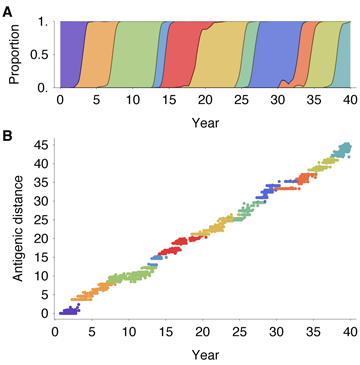
\includegraphics{figures/phenotypes}
	\caption{\textbf{Antigenic evolution over the course of the 40-year simulation}. (A) Two-dimensional antigenic phenotypes of 5943 viruses.  Each discrete virus phenotype is shown as a bubble, with bubble area proportional to the number of times this phenotype was sampled. (B) Proportion of virus population comprised of each antigenic cluster through time.  (C) Antigenic distance from initial phenotype ($x=0,y=0$) for each of 5943 virus samples relative to time of virus sampling. In (A) and (C) viruses were sampled at a constant rate proportional to prevalence and coloring was determined by clustering samples on the antigenic map in \ref{incmaptree}B.}
	\label{phenotypes}
\end{figure}

\pagebreak

%%% Figure S2: incdrift %%%
\begin{figure}[!c]
	\centering
	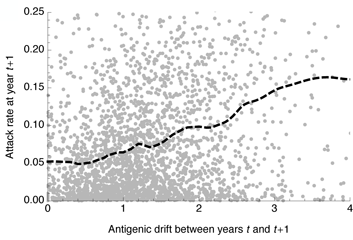
\includegraphics{figures/driftvsinc}
	\caption{\textbf{Correlation between antigenic drift and attack rate and autocorrelation of attack rate}. (A) Antigenic drift measured as the distance between the centroid of phenotypes at year $t$ and the centroid of phenotypes at year $t+1$ vs.\ annual attack rate at year $t+1$. (B) Temperate attack rate at year $t$ vs.\ temperate attack rate at year $t+1$. In both cases, measurements are taken across replicate simulations and individual pairs of measurements are shown as gray points and a locally-linear regression (LOESS) as black dashed line.}
	\label{driftvsinc}
\end{figure}

\pagebreak

%%% Figure S2: mutspectrum %%%
\begin{figure}[!c]
	\centering
	\makebox[\textwidth]{		
		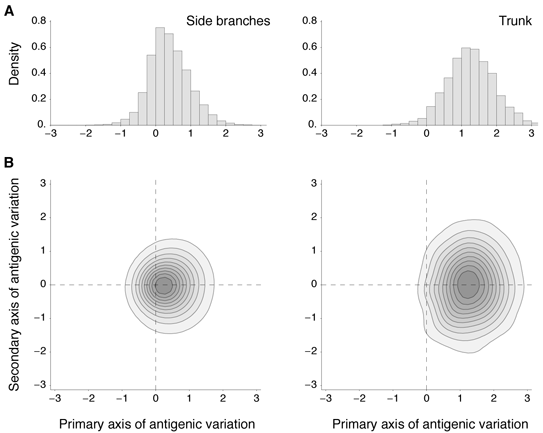
\includegraphics{figures/mutspectrum}
	}
	\caption{\textbf{Mutation spectrum in two-dimensional antigenic space of side branch mutations and trunk mutations}. (A) Histogram of mutation effects along the axis of primary antigenic variation across 80 replicate simulations.  The left panel shows the distribution of effects of side branch mutations and the right panel shows the distribution of effects of trunk mutations. (B) Smoothed two-dimensional histogram of mutation effects along the primary and secondary axes of antigenic variation across 80 replicate simulations.  Histograms were constructed from 21,405 side branch mutations and 1584 trunk mutations.}
	\label{mutspectrum}
\end{figure}

\pagebreak

%%% Figure S3: probtrunk %%%
\begin{figure}[!c]
	\centering
	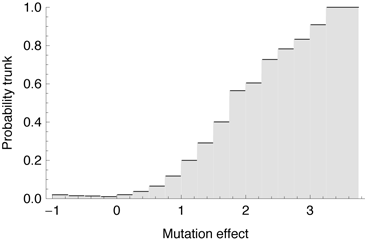
\includegraphics{figures/probtrunk}
	\caption{\textbf{Relationship between a mutation's phenotypic effect and its likelihood of being part of the trunk}. The $x$-axis represents the effect of a mutation along the line of primary antigenic variation, and the $y$-axis represents the probability that the mutation is part of the trunk.  Mutations of large effect are increasingly rare, but when they do occur are increasingly likely to be part of the trunk.}
	\label{probtrunk}
\end{figure}

\pagebreak

%%% Figure S5: waittimes %%%
\begin{figure}[!c]
	\centering
	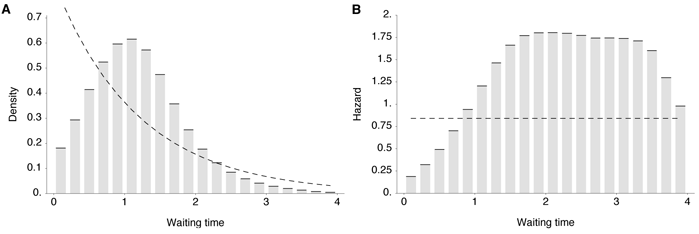
\includegraphics{figures/waittimes}
	\caption{\textbf{Observed vs.\ expected distributions of waiting times between phenotypic mutations along genealogy trunk.} (A) Histogram bins show the observed distribution of waiting times in years across 80 replicate simulations representing 1584 mutations.  The mean of this distribution is 1.76 years.  The dashed line shows the Poisson process expectation of exponentially distributed waiting times.  (B) The density distribution of waiting times is transformed into a hazard function, representing the rate of trunk mutation after a specific waiting time.  The dashed line shows the memoryless hazard function of the Poisson process expectation.}
	\label{waittimes}
\end{figure}

\pagebreak

%%% Figure S8: h1n1_mut %%%
\begin{figure}[!c]
	\centering
	\makebox[\textwidth]{
		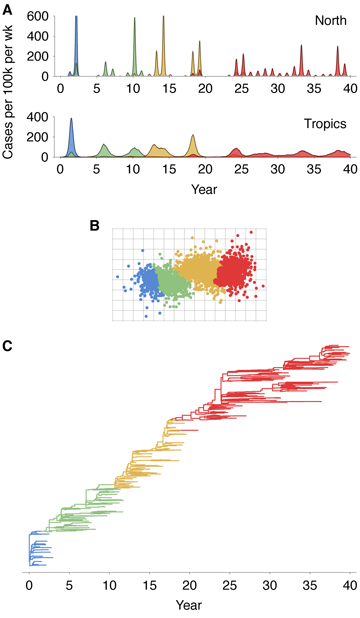
\includegraphics{figures/h1n1_mut}
	}
	\caption{\textbf{Simulation results showing epidemiological, antigenic and genealogical dynamics for weaker mutation model}. (A) Weekly timeseries of incidence of viral infection in north and tropics regions. (B) Antigenic map depicting phenotypes of viruses sampled over the course of the simulation.  Grid lines show single units of antigenic distance. (C) Genealogical tree depicting the infection history of samples from the virus population.  Cluster assignments were used to color panels (A), (B) and (C) in a consistent fashion.  Alternative mutational parameters are $\mu = 5 \times 10^{-5}$, mean mutation size of 0.42 units and standard deviation of mutation size of 0.28 units.}
	\label{h1n1_mut}
\end{figure}

\pagebreak

%%% Figure S8: h1n1_r0 %%%
\begin{figure}[!c]
	\centering
	\makebox[\textwidth]{
		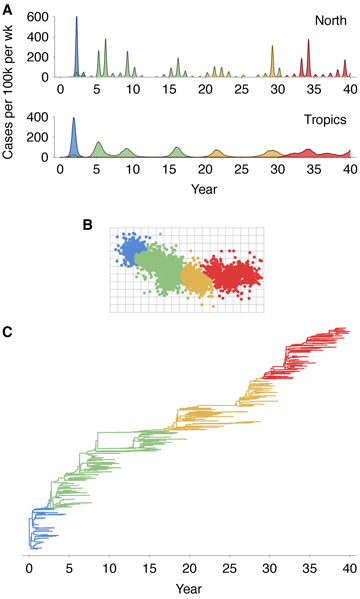
\includegraphics{figures/h1n1_r0}
	}
	\caption{\textbf{Simulation results showing epidemiological, antigenic and genealogical dynamics for lower intrinsic $R_0$}. (A) Weekly timeseries of incidence of viral infection in north and tropics regions. (B) Antigenic map depicting phenotypes of viruses sampled over the course of the simulation.  Grid lines show single units of antigenic distance. (C) Genealogical tree depicting the infection history of samples from the virus population.  Cluster assignments were used to color panels (A), (B) and (C) in a consistent fashion.  Alternative epidemiological parameters are $\beta = 0.3$ giving $R_0 = 1.5$.}
	\label{h1n1_r0}
\end{figure}

\pagebreak

%%% Figure S4: 10dgrid %%%
\begin{figure}[!c]
	\centering
	\makebox[\textwidth]{	
		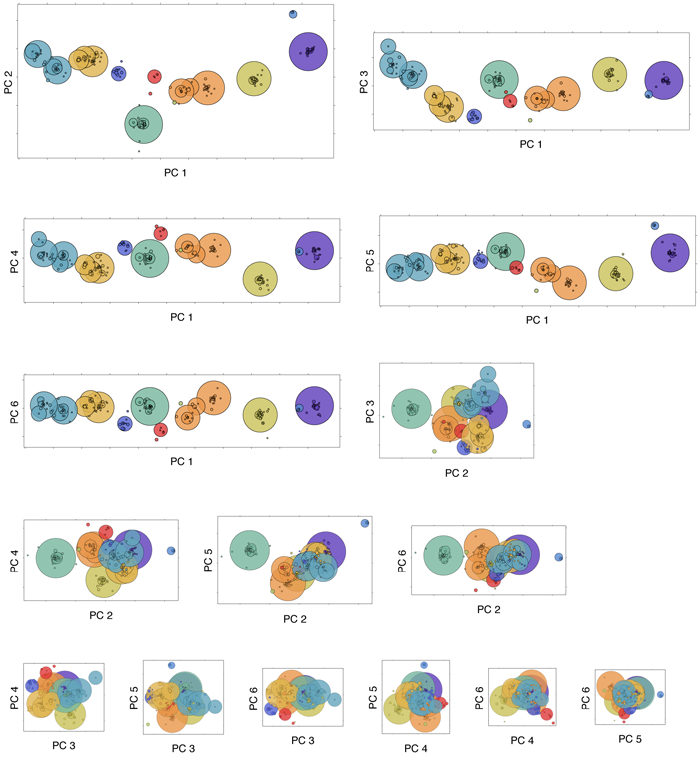
\includegraphics{figures/10dgrid}
	}
	\caption{\textbf{Principal components of antigenic variation under a 10-sphere mutation model}. Each panel shows approximately 6000 samples of antigenic phenotype over the course of a 40-year simulation.  Each phenotype is represented as a bubble, with bubble area proportional to the number of samples with this phenotype.  Bubbles are colored based on clustering the 10-dimensional antigenic phenotypes.  The original 10-dimensional space was rotated using principal components analysis to give orthogonal axes in the order of their contribution to antigenic variation.  Each panel shows a two-dimensional slice of the this rotated space.  Principal components 7--10 were left out of the figure for clarity.}
	\label{10dgrid}
\end{figure}

\pagebreak

%%% Figure 6: replicateevolfull %%%
\begin{figure}[!c]
	\centering
	\makebox[\textwidth]{	
		\includegraphics{figures/replicateevolfull}
	}
	\caption{\textbf{Antigenic phenotypes over the course of 5 years of evolution across 100 replicate simulations starting from identical initial conditions}.  Replicate simulations were initialized with the end state of the original 40-year simulation shown in \ref{incmaptree}.  The top left panel shows every antigenic phenotype present in the initial virus population.  The black point represents the population mean.  Each subsequent panel shows an additional year of evolution, with black points representing the mean antigenic phenotypes of the 100 replicate simulations and gray lines representing the history of each mean antigenic phenotype.}
	\label{replicateevolfull}
\end{figure}

\pagebreak

%%% Figure S6: replicatetimeseries %%%
\begin{figure}[!c]
	\centering
	\makebox[\textwidth]{
		\includegraphics{figures/replicatetimeseries}
	}
	\caption{\textbf{Timeseries of incidence across 100 replicate simulations with identical initial conditions.} Panels show incidence in the North, Tropics and South regions over the course of 10 years.  Solid black lines represent the median weekly incidence across the 100 replicate simulations, while gray intervals represent the interquartile range across simulations.  There is little variability for the first year of replicate simulations.  Replicate simulations were initialized with the end state of the original 40-year simulation shown in \ref{incmaptree}.}
	\label{replicatetimeseries}
\end{figure}

\pagebreak

%%% Figure S7: incmaptree_smooth %%%
\begin{figure}[!c]
	\centering
	\makebox[\textwidth]{
		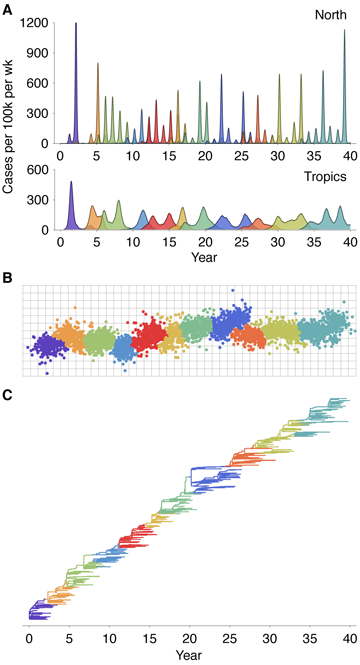
\includegraphics{figures/incmaptree_smooth}
	}
	\caption{\textbf{Simulation results showing epidemiological, antigenic and genealogical dynamics for `smoother' mutation model}. (A) Weekly timeseries of incidence of viral infection in north and tropics regions. (B) Antigenic map depicting phenotypes of viruses sampled over the course of the simulation.  Grid lines show single units of antigenic distance. (C) Genealogical tree depicting the infection history of samples from the virus population.  Cluster assignments were used to color panels (A), (B) and (C) in a consistent fashion.  Alternative mutational parameters are $\mu = 3 \times 10^{-4}$, mean mutation size of 0.6 units and standard deviation of mutation size of 0.2 units.}
	\label{incmaptree_smooth}
\end{figure}

\pagebreak

%%% Figure S8: incmaptree_rough %%%
\begin{figure}[!c]
	\centering
	\makebox[\textwidth]{
		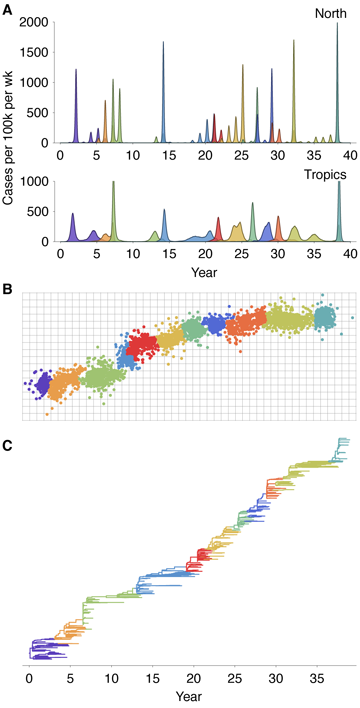
\includegraphics{figures/incmaptree_rough}
	}
	\caption{\textbf{Simulation results showing epidemiological, antigenic and genealogical dynamics for `rougher' mutation model}. (A) Weekly timeseries of incidence of viral infection in north and tropics regions. (B) Antigenic map depicting phenotypes of viruses sampled over the course of the simulation.  Grid lines show single units of antigenic distance. (C) Genealogical tree depicting the infection history of samples from the virus population.  Cluster assignments were used to color panels (A), (B) and (C) in a consistent fashion.  Alternative mutational parameters are $\mu = 5 \times 10^{-5}$, mean mutation size of 0.7 units and standard deviation of mutation size of 0.5 units.}
	\label{incmaptree_rough}
\end{figure}
